\chapter{Results}
\label{chap:results}

\section{Summary}

\subsection{accuracy}

\begin{table}[ht]
    \caption{Mobility $cm^{2}/Vs$} % title of Table
\centering % used for centering table
\begin{tabular}{c c c c} % centered columns (4 columns)
\hline\hline %inserts double horizontal lines
Software & Amorphous & Semi-crystalline & Crystalline \\ [0.5ex] % inserts table
%heading
\hline % inserts single horizontal line
ORCA & 1 & 1 & 1 \\ % inserting body of the table
PySCF & 1 & 1 & 1 \\ [1ex] % [1ex] adds vertical space
\hline %inserts single line
\end{tabular}
\label{table:nonlin} % is used to refer this table in the text
\end{table}

\subsection{Sensitivity}

\subsubsection{dcut}

A parameter introduced in the kmc algorithm dcut that trims the fat off of the voronoi neighlist builing.
As can seen from the figure, two points (chromophores), can share cell edges despite being rather far apart. We
therefore, further remove pairs from the neighborlist if they are far enough apart such that it is justifyable
to assume they dont interact electronically enough to effect to charge mobility calc. This parameter will
dependend on the material under investigation as was as the size of the individual chromophores. We tested the
sensitivity of the algorithm to the value (dcut). The [zoomed figure] Shows a example dcut radaii. Note that
the z-direction has been collaped, and the distinces dont necessarily correlate to the distance
between chromophores in the system. The figure shows the effect of cutoff distance on value of
16 calculated mobility. there is a diminishing returns around dcut10.


\begin{table}[ht]
    \caption{dcut sensitivity}
\centering % used for centering table
\begin{tabular}{c c c c c c c c} % centered columns (4 columns)
\hline\hline %inserts double horizontal lines
dcut & 4 & 6 & 8 & 10 & 12 & 14 & 16 \\ [0.5ex] % inserts table
%heading
\hline % inserts single horizontal line
 pairs & 4 & 6 & 8 & 10 & 12 & 14 & 16 \\ % inserting body of the table
$\mu_{0}$ & 4 & 6 & 8 & 10 & 12 & 14 & 16 \\ [1ex] % [1ex] adds vertical space
\hline %inserts single line
\end{tabular}
\label{table:dcut-sense} % is used to refer this table in the text
\end{table}

\begin{figure}
  \center
  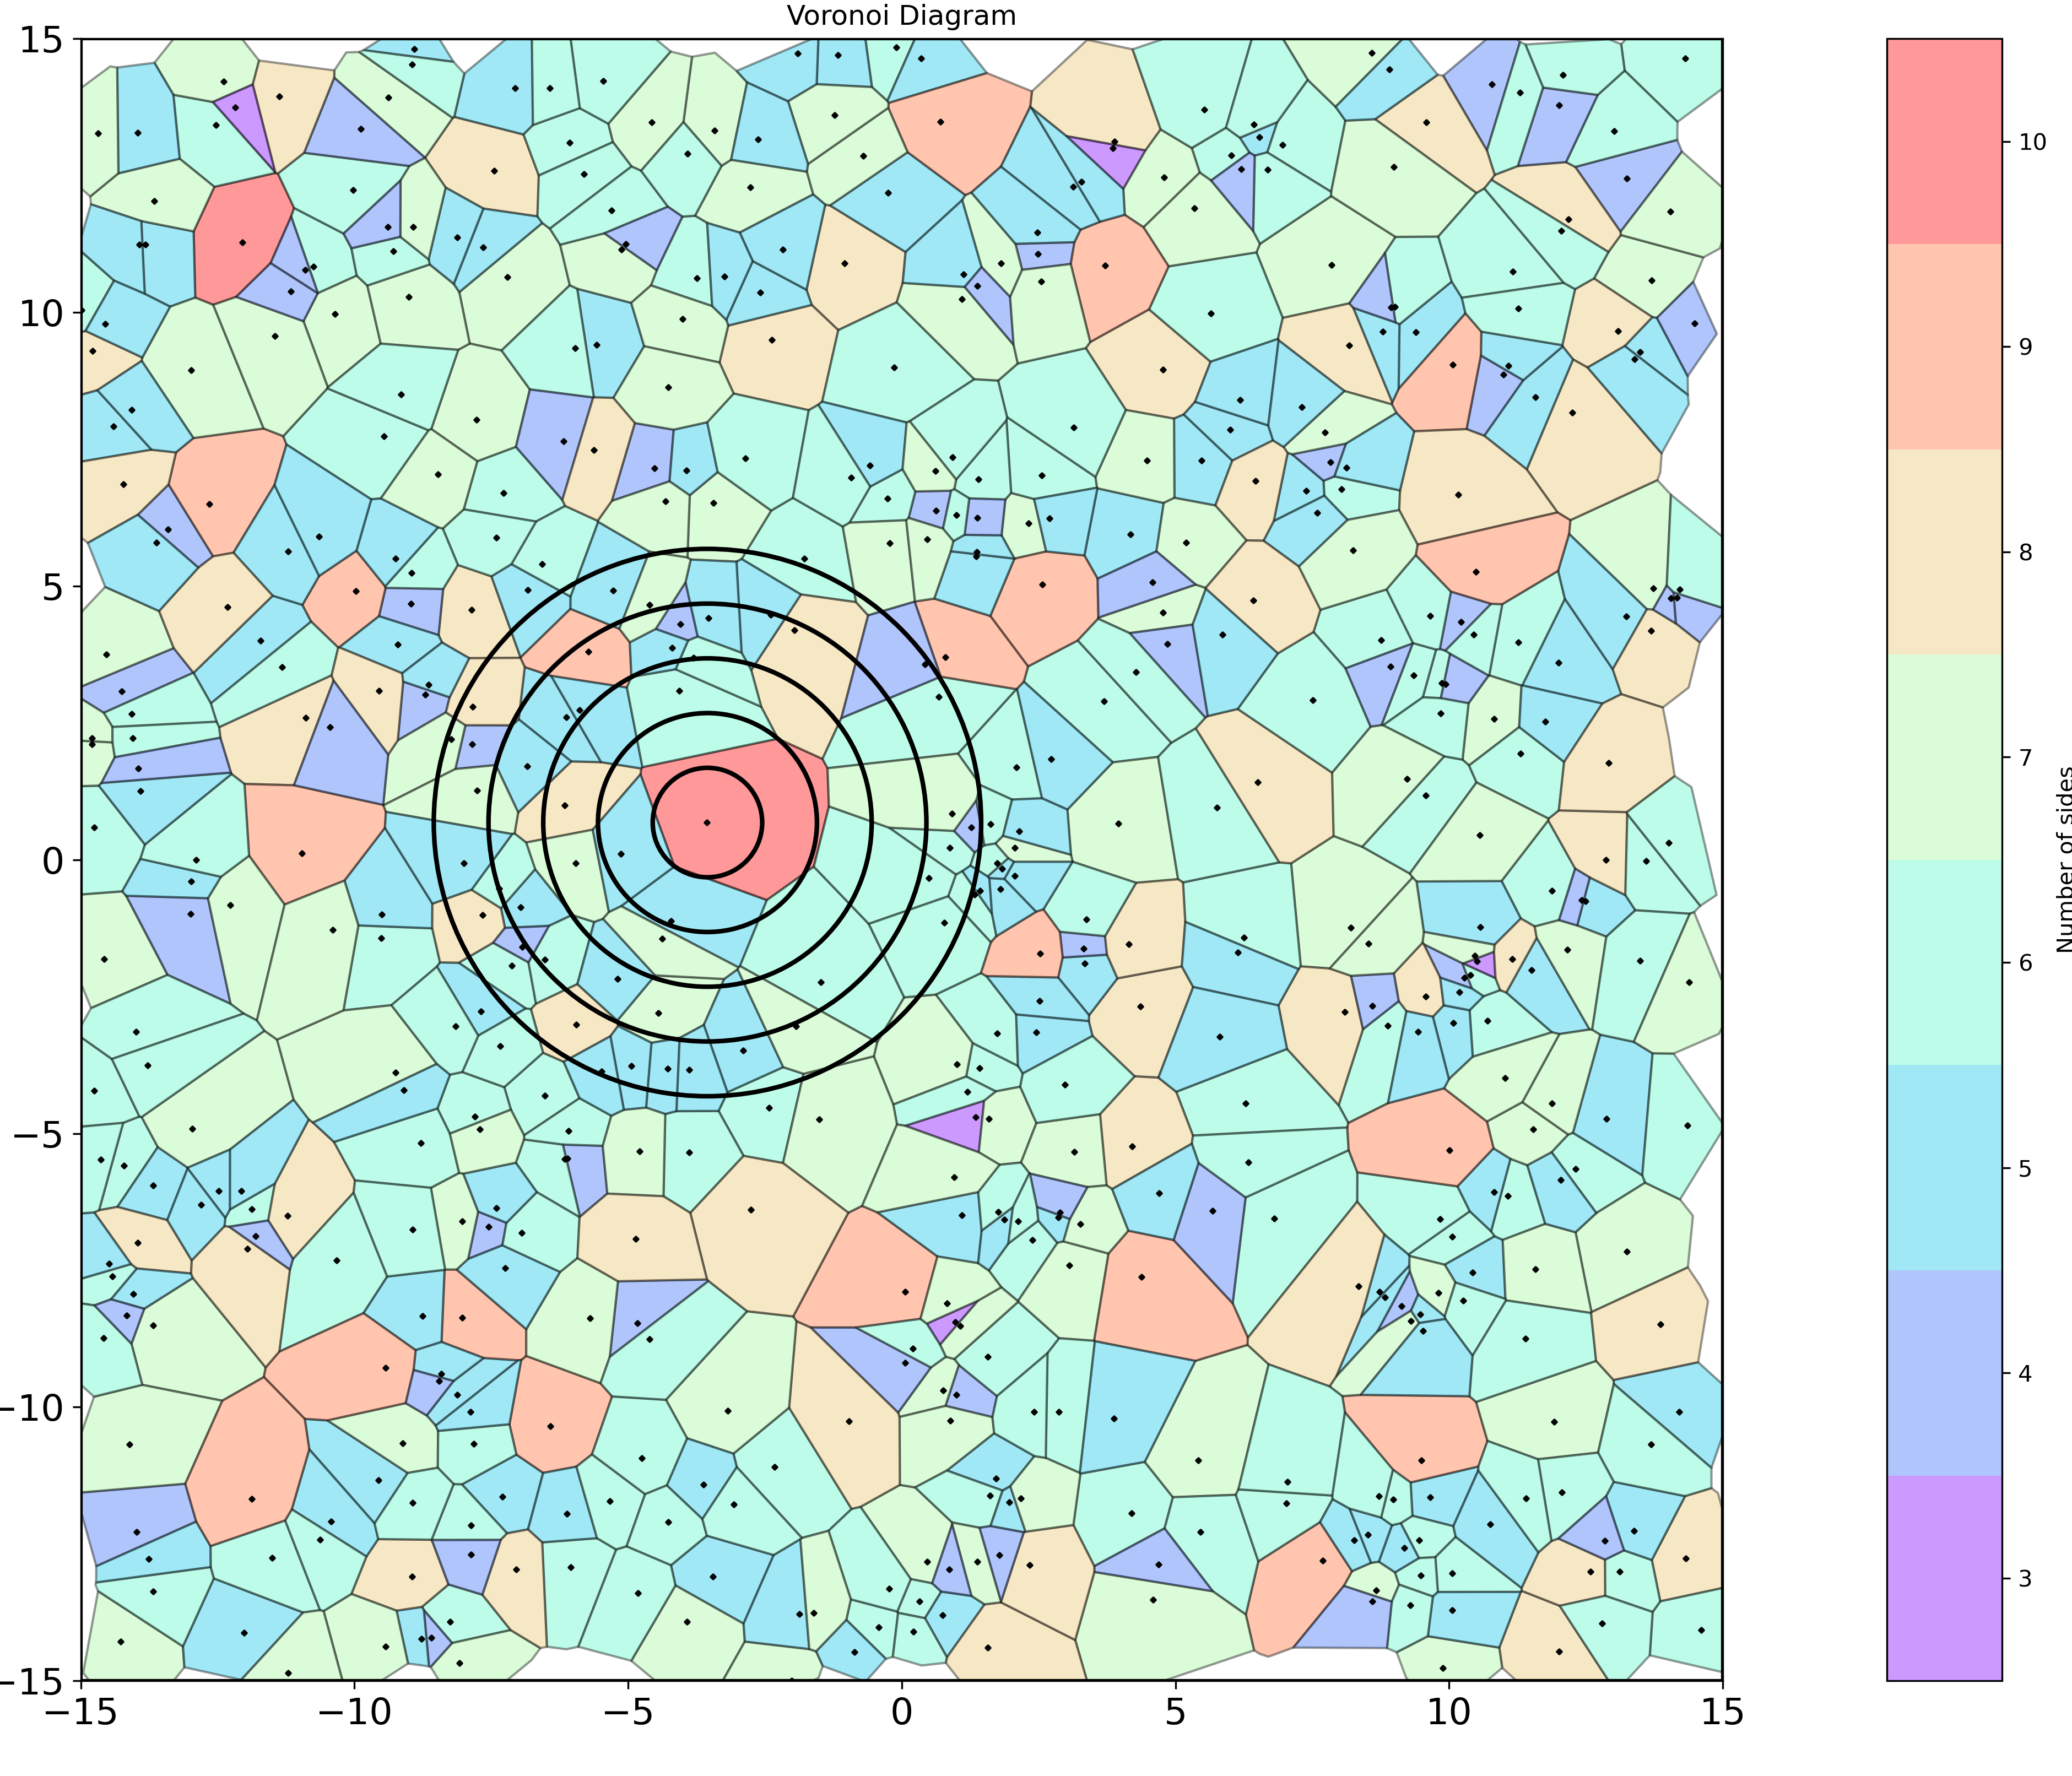
\includegraphics[width=\linewidth, height=\textheight,keepaspectratio]{figures/crystalline_voronoi_d_cut_circles.png} 
  \caption{dcut visual}
  \label{fig:dcut}
\end{figure}


\subsubsection{Reorganization energy}
Marcus's nonadiabatic electron transfer theory allows us to model charge transfer as two
intersecting parabolic potential energy surfaces. In this work, the parabalas represent the potential energy surface
of the dimer created by a pair of chomophores with a charge injected on either chromophore.  oThe reorganization energy constitutes a 
\begin{figure}
  \center
  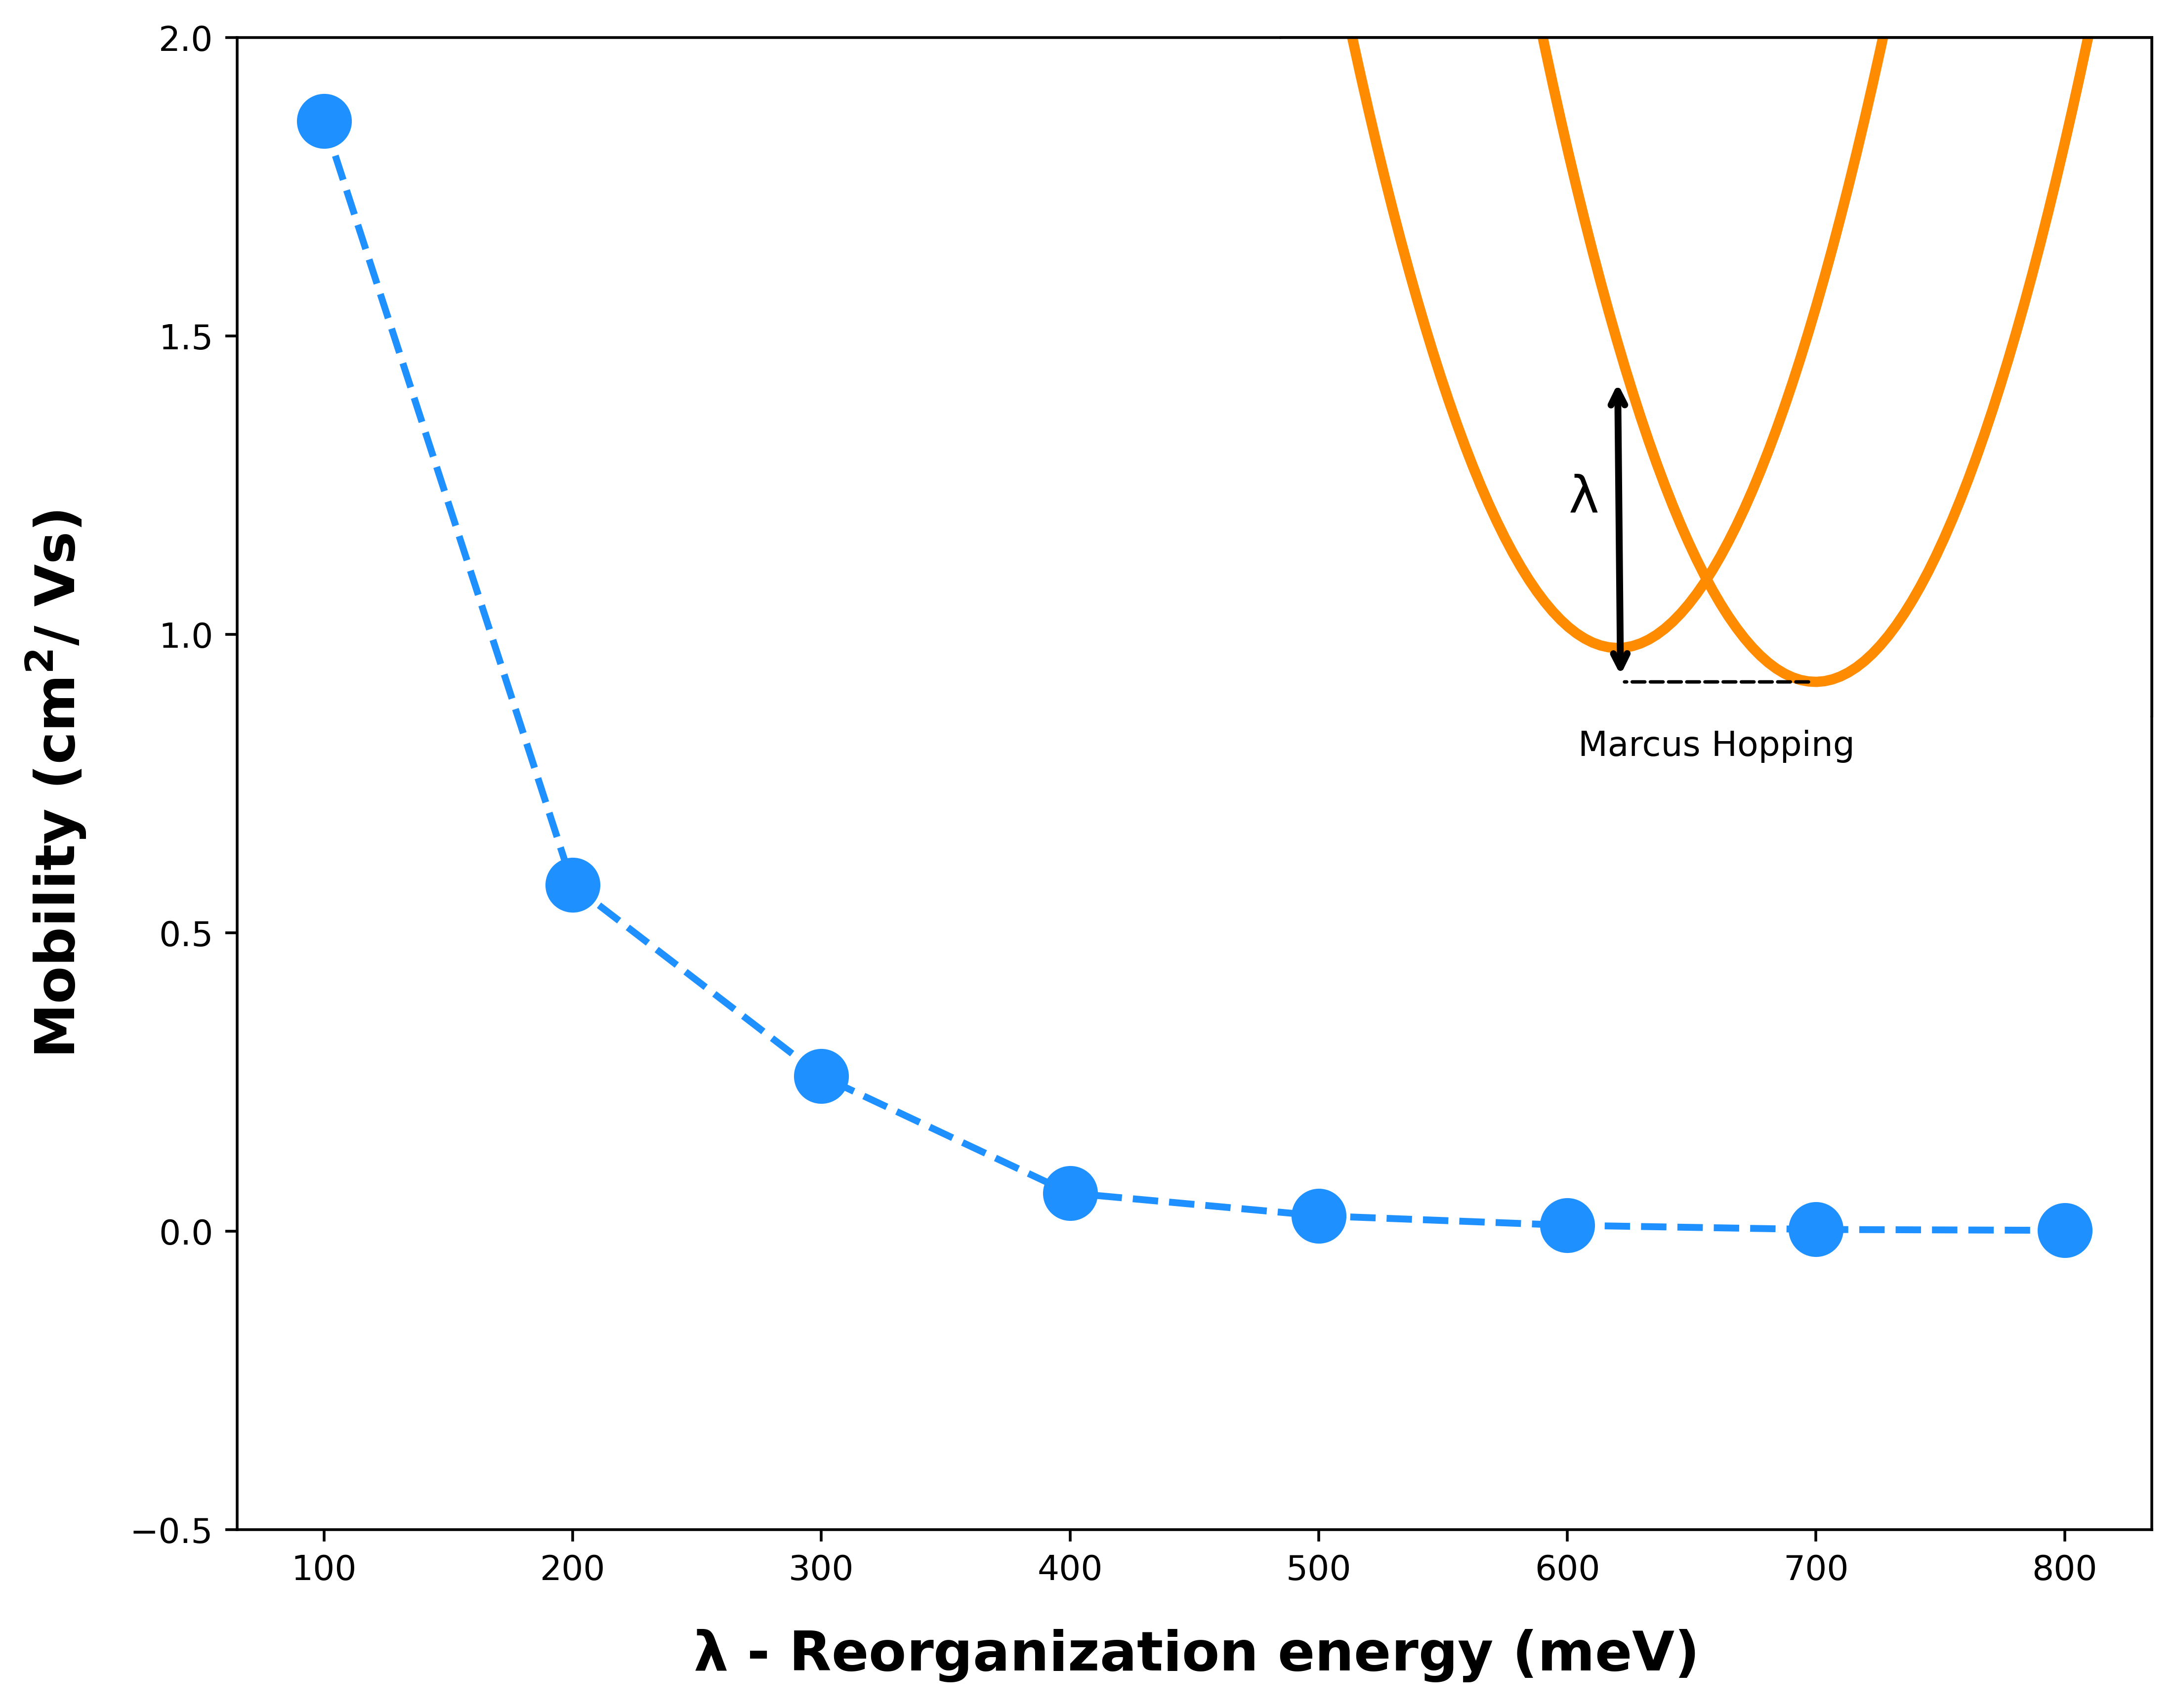
\includegraphics[width=\linewidth, height=\textheight,keepaspectratio]{figures/reorg.png} 
    \caption{The results of running 8 KMC simulations with reorganization energy 100-800 meV}
  \label{fig:reorg}
\end{figure}

\subsubsection{lifetimes}

\subsection{Improvements}
Dynamic disorder does effect charge mobility (CT in high mobility conjugated polymers) with every pico second
may have a 10-20\% fluxuation in TI. 
In our kmc algorithm we could incorperate the rates of other events like recombination.

The computational bottle neck of simulation charge mobility is also the most theoreticaly challenging.
Estimating the TI for each pair of cromophores. A future improvement to MorphCT will be accelerating this step
with Machine learning techniques. Musil et al. have shown that ML could produce a 90 \% decrease in
computationl effort \cite{Musil2018}

Something to do is allow morphct as to figure out what to do with donor accpeter mixtures. It would be pretty
easy to run asyncronously on the donor/acceptor materials and compare. this could be a measure of morphology.
If you run pure donor and pure acceptor and you got mobities, if on of those drops in the mixed morph more
that the other you probably dont have a nice domain for BHJ.

%%% Local Variables: 
%%% mode: latex
%%% TeX-master: "BSUmain"
%%% End: 
